\section{Scheduling with Unknown Arrival Types: The Nested WAIT Algorithm}
\label{sec:nested_wait}

In the previous section, we introduced the WAIT algorithm for scheduling inference tasks with known prompt types, achieving near-optimal throughput. However, real-world LLM inference systems often encounter prompts whose types—and consequently their output lengths—are unknown upon arrival. To address this challenge, we propose the \textit{Nested Waiting for Accumulated Inference Threshold} (Nested WAIT) algorithm, which extends the WAIT framework to manage stochastic arrivals with unknown types.

\subsection{Algorithm Overview}

To begin with, note that adapting algorithms for known lengths by assuming worst-case lengths is inefficient. For example, with two prompt types (input length 1, arrival rates equal), one with output length 1 and another 10,000, assuming 10,000 for all yields memory utilization as low as \( 1/5000 \). Therefore, the Nested WAIT algorithm extends the WAIT policy by introducing a nested structure to manage prompts with unknown output lengths. The mechanism tries to distinguish different types of arrivals by iterating step by step, rather than assuming or guessing this information at the beginning. 

We assume that while the specific type of each arriving prompt is unknown, the possible output lengths follow a known distribution, inferred from the inference service. Formally, let the output length of type \( j \) be \( l_j \) after the prefill phase and \( l_j' \) after the decode phase, with \( l_1' < l_2' < \dots < l_m' \). The algorithm organizes the inference process into \( m \) nested segments, each corresponding to cumulative processing stages up to these potential output lengths. It is parameterized by \( m \) thresholds \( \pi = [n_1, \dots, n_m] \), where \( n_i \) corresponds to the \( i \)-th segment. The core logic determines prompt types upon completing each segment.

The process divides into \( m \) segments. In the first segment, the total arrival rate is \( \lambda_1 + \cdots + \lambda_m \), covering prompts at stages \( 0, 1, \dots, l_1' \). After \( l_1' + 1 \) iterations, all prompts in segment 1, except those of type 1, advance to the second segment, spanning stages \( l_1' + 1, \dots, l_2' \). After \( l_2' - l_1' \) iterations, all prompts in segment 2, except those of type 2, proceed to segment 3. This continues for subsequent segments. If the number of prompts for the \( i \)-th segment is insufficient, processing pauses for that segment and all subsequent ones, retaining their KV caches on the GPU for future use. In that case, we will batch exact $n_j$ prompts at each stage in segment $j,\,\forall 0\le j\le i-1$ and perform one iteration. Since there are new arrivals with output length not smaller than $l_i$ in future, we expect segment $i$ to resume joining in the batch very soon. Algorithm \ref{alg:nested_wait} formalizes this procedure, and Figure \ref{fig:nested_wait} illustrates the pipeline. For simplicity, we assume \( l_1 = l_2 = \dots = l_m \) (identical prefill output lengths), though the general case extends similarly to Algorithm \ref{alg:wait}: segment groups are formed by prefill output lengths, and Nested WAIT runs independently for each group. Notably, the number of output lengths, \( m \), minimally impacts performance, which depends primarily on total arrival rates, as shown later. The number of segments can also differ from \( m \), while still retaining near-optimal guarantees under similar conditions. We leave the discussion in Section \ref{sec:extension}.

\begin{figure}[h]
    \centering
    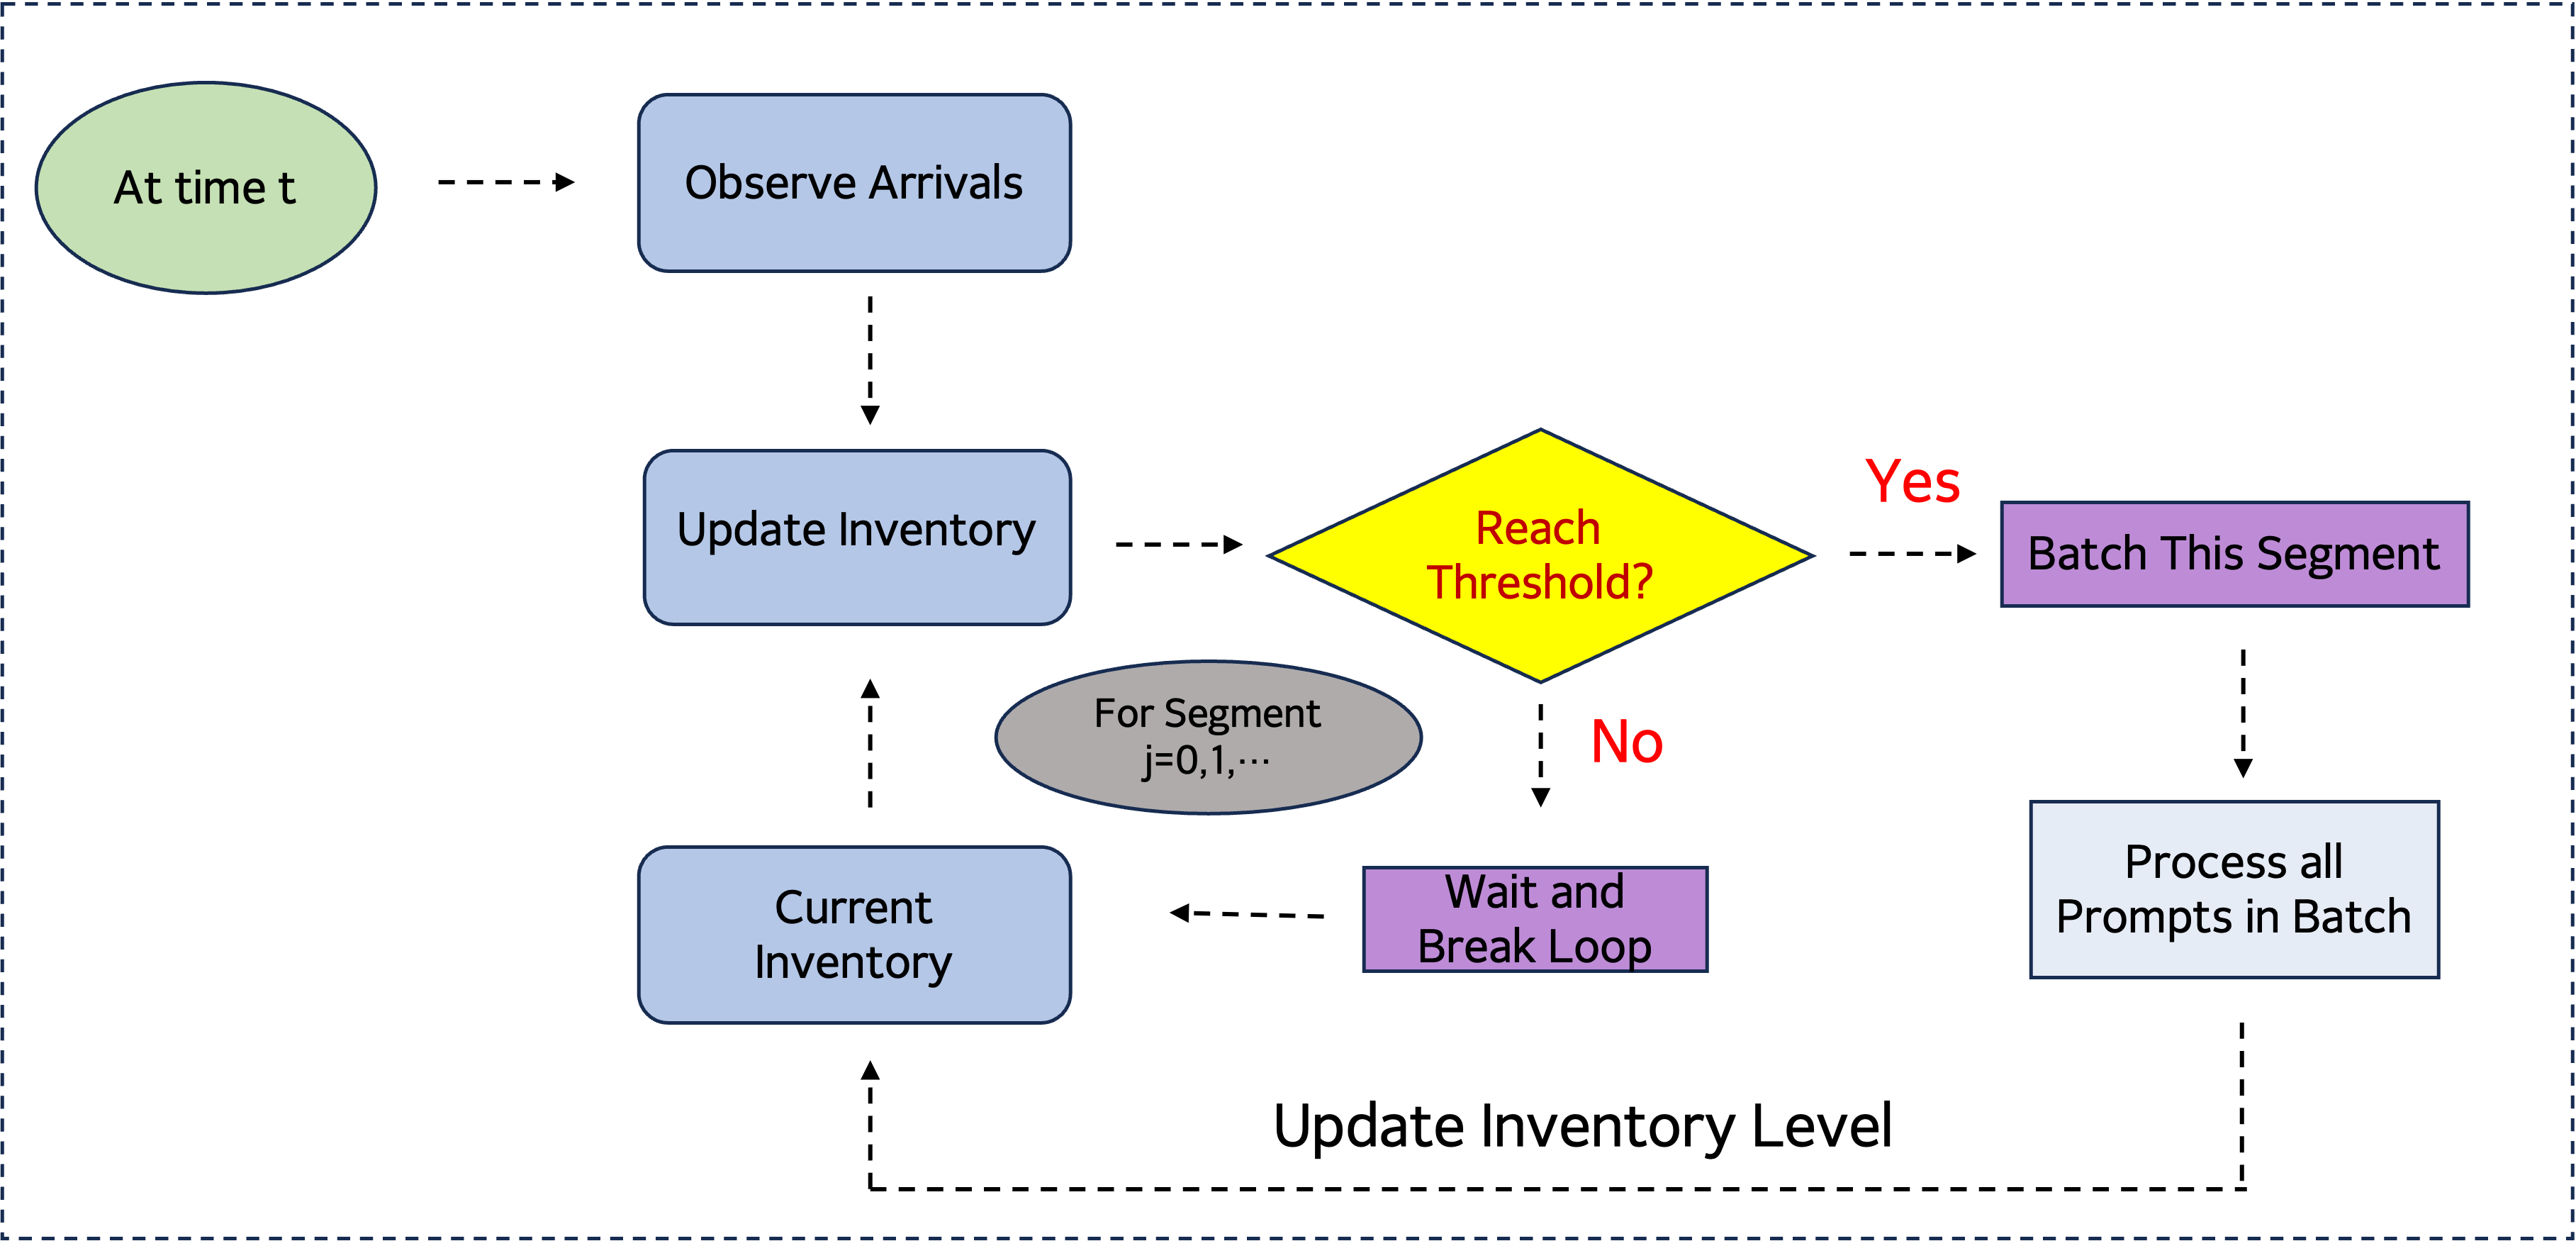
\includegraphics[width=0.9\linewidth]{fig_nestedWAIT.png}
    \caption{Pipeline of the Nested WAIT Algorithm}
    \label{fig:nested_wait}
\end{figure}
To further illustrate how our Nested WAIT works, consider a simplified scenario with two prompt types, both having the same initial input length \( l \), but differing in decode length, with \( l_1' < l_2' \). While prompt types are indistinguishable at arrival, they become identifiable after one decode iteration.  To accommodate this, the Nested WAIT algorithm partitions processing into two segments. \textbf{Segment 1} includes all prompts at stages \( 0, 1, \dots, l_1' \), and thus contains both types of prompts immediately after arrival. \textbf{Segment 2}, in contrast, includes only type-2 prompts at later stages \( l_1'+1, \dots, l_2' \), once type-1 prompts have completed. The effective arrival rate for Segment 1 is \( \lambda_1 + \lambda_2 \), while Segment 2 receives prompts at a reduced rate \( \lambda_2 \), delayed by one decode step. Figure~\ref{fig:nested_wait_example} visualizes the algorithm in action. At time \( t=0 \), prompts \( P1 \) and \( P2 \) arrive but are insufficient to trigger processing, as Segment 1 has fewer than 3 prompts. At \( t=1 \), \( P3 \) arrives, satisfying the Segment 1 threshold, and the batch is processed. Since these prompts have just begun decoding, none qualify for Segment 2. At \( t=5 \), a new wave of prompts (\( P4 \), \( P5 \)) arrives, again below the threshold. By \( t=7 \), the threshold is met with \( P6 \), \( P7 \), and processing proceeds. Now, \( P3 \), having reached a deeper decode stage, transitions to Segment 2. However, since the Segment 2 threshold is still unmet, only Segment 1 is processed. Finally, at \( t=14 \), enough prompts have advanced into Segment 2 (\( P3 \), \( P5 \), \( P6 \), etc.) to satisfy both segment thresholds. At this point, the Nested WAIT algorithm jointly schedules both segments, maximizing GPU efficiency by batching according to type-specific readiness. This example illustrates how the algorithm defers processing to ensure type separation and stage-aligned batching, achieving high utilization while respecting decode-stage heterogeneity and unknown output.


\begin{figure}[h]
    \centering
    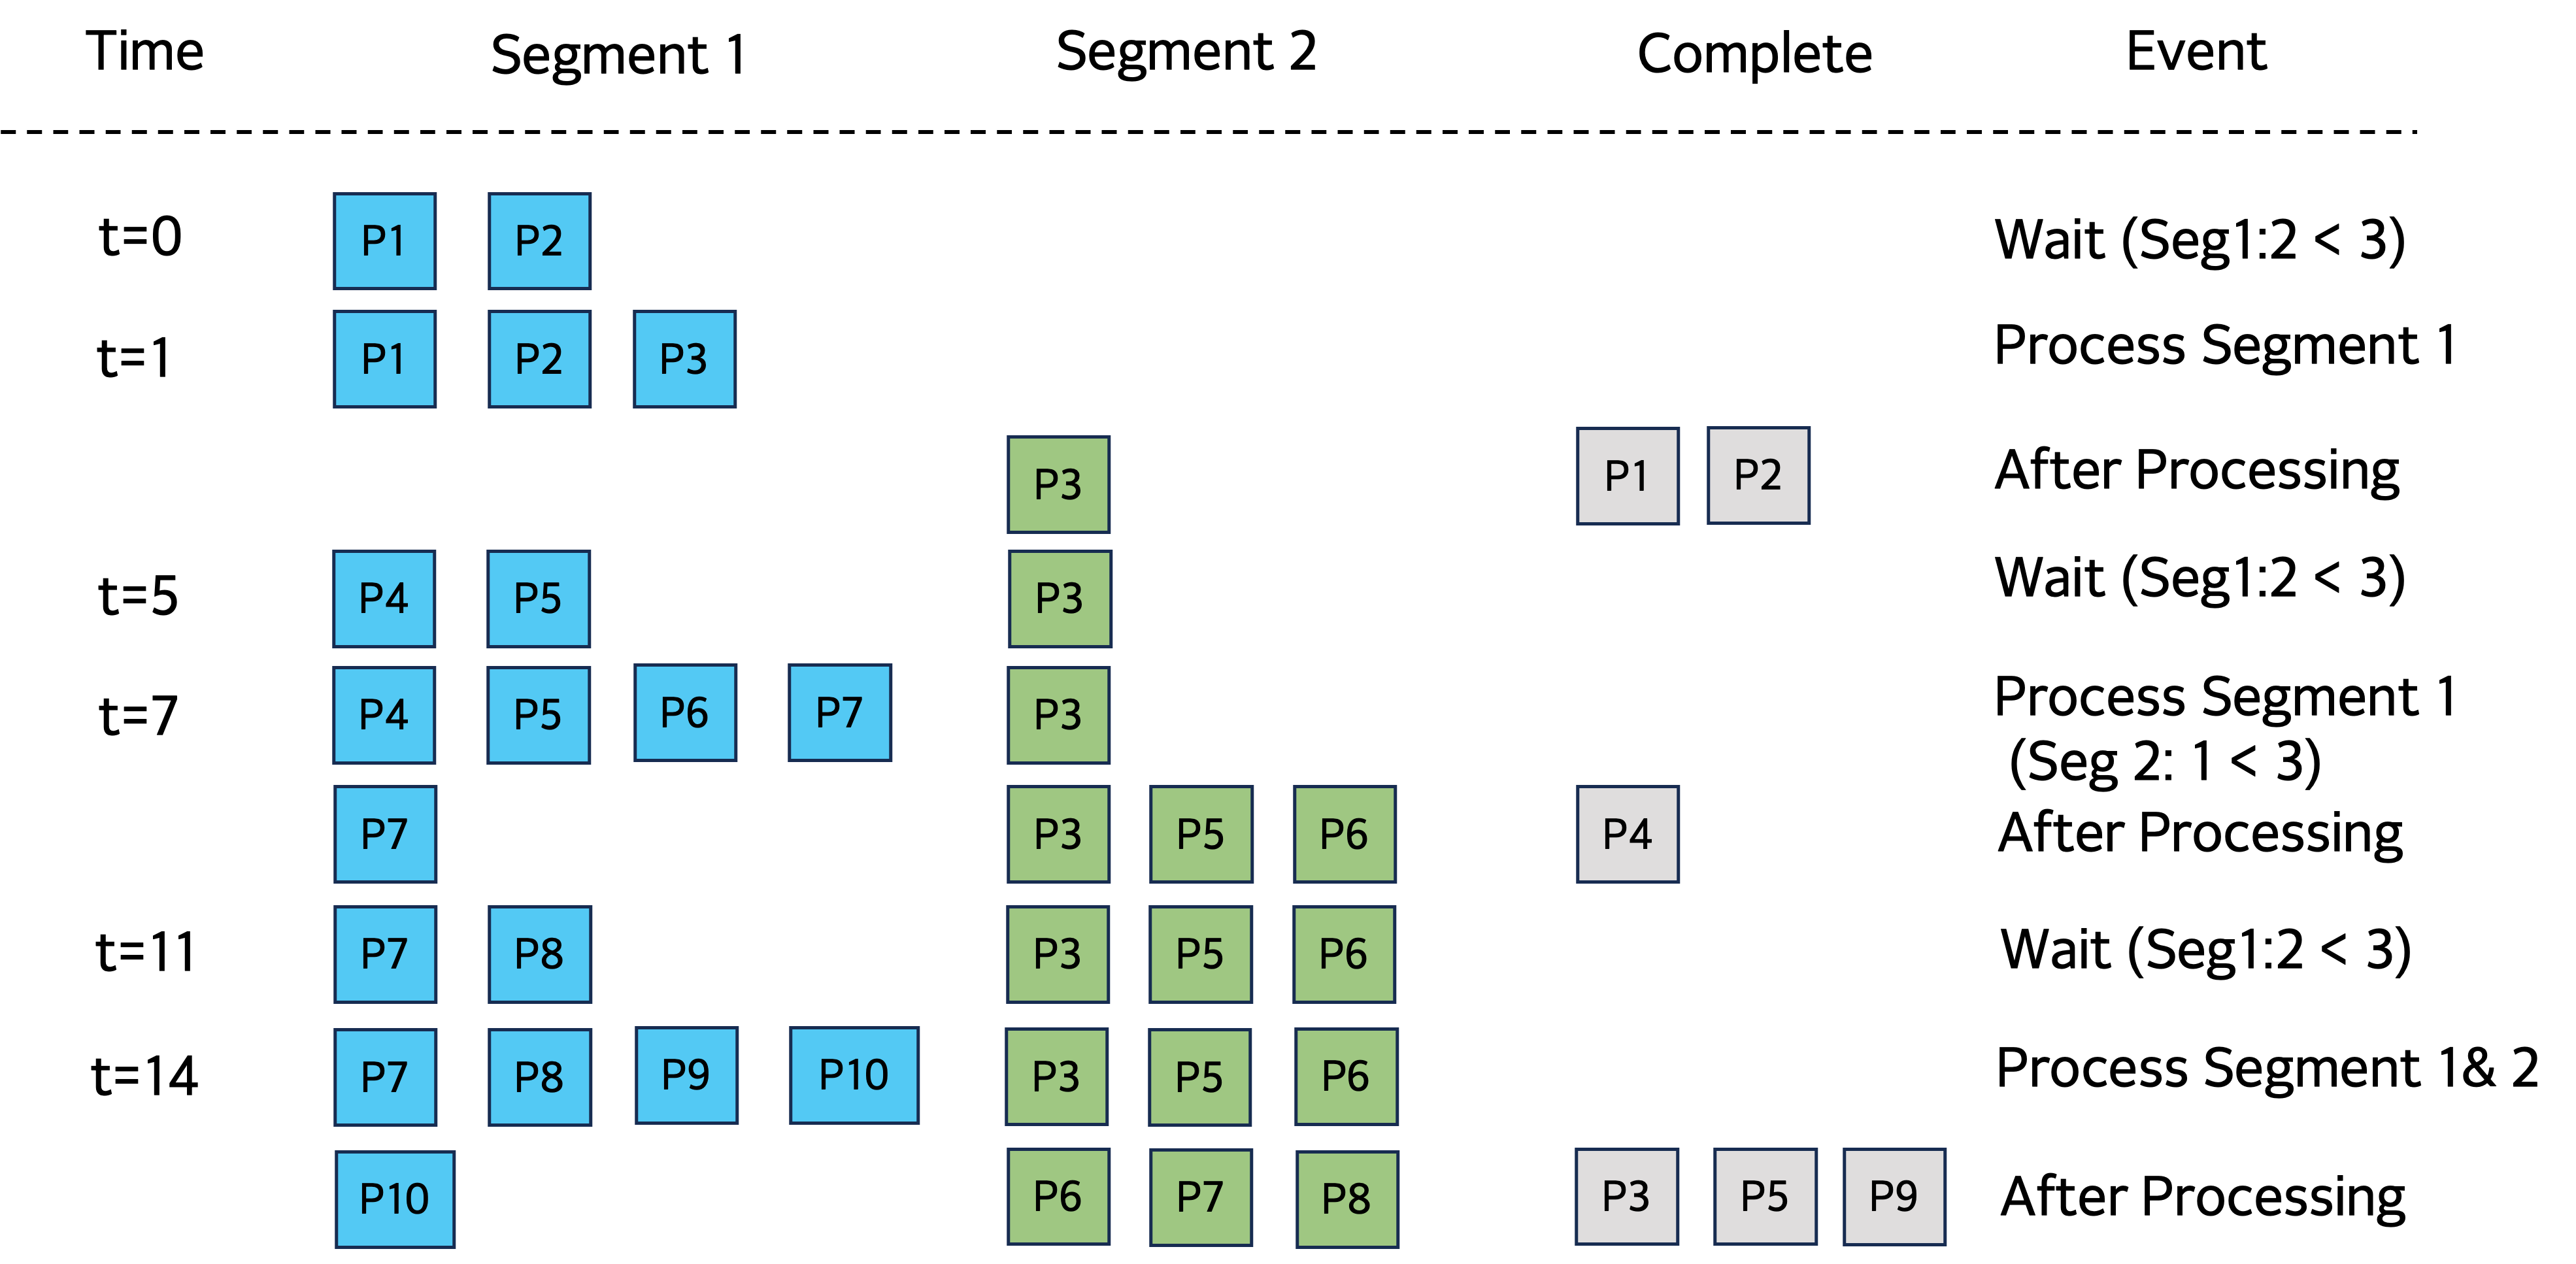
\includegraphics[width=0.9\linewidth]{fig_nestedWAIT_example.png}
    \caption{Example of the Nested WAIT Algorithm}
    \label{fig:nested_wait_example}
\end{figure}

\begin{algorithm}[h]
\caption{Nested WAIT: Nested Waiting for Accumulated Inference Threshold}
\label{alg:nested_wait}
{\small\linespread{1.0}\selectfont
\begin{algorithmic}[1]
\Require Memory capacity \( C \), arrival rates \( \lambda_j \) for \( j \in [m] \), thresholds \( n_i \) for segments \( i \in [m] \)
\Require Output lengths \( l_1' < l_2' < \cdots < l_m' \) for prompt types \( j \in [m] \)
\State Initialize segment inventories \( n_{i,k} \gets 0 \) for all \( i \in [m], k \in \{\sum_{j=1}^{i-1} l_j', \dots, \sum_{j=1}^{i} l_j' - 1\} \)
\State Initialize event queue
\State Set current time \( t \gets 0 \)
\While{True}
    \State Wait for the next event (arrival or batch completion)
    \If{event is an arrival}
        \State Update inventory: \( n_{1,0} \gets n_{1,0} + 1 \)  \Comment{New prompts start in segment 1, stage 0}
    \ElsIf{event is a batch completion for segment \( i \)}
        \State Update inventory: For each stage \( k \) in segment \( i \), \( n_{i,k} \gets n_{i,k} - \min\{n_i, n_{i,k}\} \)
        \State Advance prompts: Move \( \min\{n_i, n_{i,k}\} \) prompts from stage \( k \) to \( k+1 \) within segment \( i \)
        \If{prompts reach stage \( l_i' + 1 \)}
            \If{\( i < m \)}
                \State Move incomplete prompts to segment \( i+1 \), stage \( l_i' + 1 \) \Comment{Prompts are of types \( \geq i+1 \)}
            \Else
                \State Clear KV caches for completed prompts
            \EndIf
        \EndIf
    \EndIf
    \State Find the largest \( i \) such that \( n_{i', \sum_{j=1}^{i'-1} l_j'} \geq n_{i'} \) for all \( i' = 1 \) to \( i \)
    \If{such an \( i \) exists}
        \State Form batch \( B \) from segments \( i' \leq i \) by selecting \( \min\{n_{i'}, n_{i',k}\} \) prompts at each stage \( k \)
        \State Process batch \( B \), keep prompts outside the batch waiting and do not delete their KV caches
    \EndIf
\EndWhile
\end{algorithmic}
}
\end{algorithm}

\subsection{Main Theorem}
\label{subsec:nested_main_theorem}

We evaluate Nested WAIT’s performance under conventional heavy-traffic regimes (Section \ref{sec:wait}). Unknown prompt types increase complexity, as variable output lengths affect memory and processing times. The primary metric is average throughput, \( \throughput^{(\zeta, \pi)} \), where \( \zeta \) is the scaling parameter and \( \pi \) is the Nested WAIT policy. We also provide theoretical results for average latency \( \Latency^{(\zeta, \pi)} \) and time-to-first-token \( \TTFT^{(\zeta, \pi)} \).

To achieve an asymptotic performance gap of \( o(1) \), memory \( M \) must exceed the equilibrium memory in Equation \eqref{eq:memory_multi2}, in order to mitigate overflow risks due to initially unknown output lengths. The following proposition shows that the worst-case throughput gap between any non-predictive policy unaware of arrival types and the fluid throughput (Equation \eqref{eq:throughput_fluid}) is at least \( \Omega(1) \).

\begin{proposition}
\label{prop:unknown_lower_bound}
When memory capacity \( C \) equals the equilibrium memory \( M^* \), there exists an instance where any online non-predictive policy \( \pi \), unaware of prompt types upon arrival, incurs a throughput gap \( \throughput^* - \mathbb{E}[\throughput^{(\zeta, \pi)}] = \Omega(1) \).
\end{proposition}

Intuitively, with \( C = M^* \), ignorance of output lengths risks under-utilization or overflow after each iteration. Overflow forces restarts, reducing efficiency. Both scenarios yield a throughput gap of \( \Omega(1 / (\zeta T)) \), accumulating to \( \Omega(1) \) over time. See Appendix \ref{sec:proof_unknown_lower_bound} for a detailed proof.



Similar to Equation \eqref{eq:wait_thresholds}, we define \( \Delta T_{[1,\dots,m]}(n_1, \dots, n_m) \) as the time cost per iteration with exactly \( n_i \) prompts per stage in segment \( i \), for all \( i \in [1, \dots, m] \). Thresholds must satisfy:
\begin{equation}
    \label{eq:nested_wait_thresholds}
    \Delta T_{[1,\dots,m]}(n_1, \dots, n_m) \leq \frac{n_1}{\sum_{j=1}^m \lambda_j}, \quad \frac{n_{i+1}}{\sum_{j=i+1}^m \lambda_j} > \frac{n_i}{\sum_{j=i}^m \lambda_j}, \quad \forall i = 1, 2, \dots, m-1.
\end{equation}

Additionally, we define the memory usage when running iteration with exactly \( n_i \) prompts per stage in segment \( i \), for all \( i \in [1, \dots, m] \) as:
\begin{align}
    \label{eq:nested_wait_memory}
    M^\pi = \sum_{j=1}^m n_j \left( l + \frac{l_1' + \cdots + l_j'}{2} \right) \cdot (l_j' - l_{j-1}'), \quad l_0' = 0.
\end{align}

The following key theoretical result demonstrates Nested WAIT’s asymptotic optimality under heavy-traffic conditions with unknown prompt types, given thresholds \( \pi = [n_1, \dots, n_m] \) satisfying Equation \eqref{eq:nested_wait_thresholds}.

\begin{theorem}
\label{thm:nested_wait_heavy_traffic}
Assume thresholds \( \pi = [n_1, \dots, n_m] \) satisfy Equation \eqref{eq:nested_wait_thresholds}, and memory \( M \) satisfies:
\begin{align}
\label{eq:nested_wait_memory_total}
    M^{(\zeta,\pi)} \geq M^\pi + \sum_{j=2}^m (l + l_{j-1}') n_j + \sum_{j=2}^m (l + l_{j-1}') \theta_j^{-1} \ln\left( \frac{m \zeta T}{\delta} \right) = O\left( 2M^\pi + \sum_{j=1}^m (l + l_{j-1}') \ln\left( \frac{m \zeta T}{\delta} \right) \right),
\end{align}
where \( \theta_j \) is defined in \arc{Add reference to equation}. Then:
\begin{align*}
&\throughput^* - \mathbb{E}\left[ \throughput^{(\zeta, \pi)} \right] = O\left( (\zeta T)^{-1} \right), \\
&\mathbb{E}\left[ \Latency^{(\zeta, \pi)} \right] = O(1), \quad \mathbb{E}\left[ \TTFT^{(\zeta, \pi)} \right] = O(1).
\end{align*}
Moreover, memory is not exceeded with probability at least \( 1 - \delta \) over the time horizon.
\end{theorem}

The proof relies on constructing a coupling process that dominates the true dynamics with more tractable transition kernel. We can then adopt analytic tools for Lindley process (see e.g. \cite{hill1982comparisons}) and Doob's maximal inequality for submargtingale to establish the performance gap. See Appendix \ref{appendix::proof of nested_wait_heavy_traffic} for details.

There are three notable observations: (i) The algorithm's performance exhibits little dependence on the number of prompt types \( m \); instead, it is primarily determined by the arrival rates and output lengths. For large \( m \) (e.g., output lengths \( \{1, 2, \dots, m\} \)), employing descending thresholds \( n_1 > n_2 > \dots > n_m \) and batching up to \( n_i \) prompts per stage remains effective when arrival rates are moderate, as indicated by condition~\eqref{eq:nested_wait_thresholds}. (ii) The memory requirement given in~\eqref{eq:nested_wait_memory_total} is generally dominated by the first term \( M^\pi \). Further details and numerical support are provided in Section~\ref{sec:experiments}. (iii) As previously discussed, the segment structure can be extended from \( m \) segments to an arbitrary number \( L \). Algorithm~\ref{alg:nested_wait} retains asymptotic optimality, provided similar conditions to those specified in~\eqref{eq:nested_wait_thresholds} are satisfied. Additional discussion on this generalization is presented in Section~\ref{sec:extension}.